\documentclass[11pt,a4paper]{article}
\usepackage[utf8]{inputenc}
\usepackage[T1]{fontenc}
\usepackage{amsmath,amssymb}
\usepackage{graphicx}
\usepackage{booktabs}
\usepackage{hyperref}
\usepackage[margin=2.5cm]{geometry}
\usepackage{xcolor}
\usepackage{float}
\usepackage{caption}
\usepackage{subcaption}
\usepackage{textcomp}
\usepackage{multirow}

\title{AI Text Slop: A Quantitative Study of Stylistic Convergence Across Six Language Models in Japanese Technical Writing}

\author{Ken Imoto\\
Propel-Lab\\
\texttt{imoto@propel-lab.co.jp}\\
\url{https://kenimoto.dev}}

\date{March 2026}

\begin{document}

\maketitle

\begin{abstract}
Large Language Models (LLMs) are increasingly used for content generation, yet the resulting text often exhibits detectable stylistic patterns---a phenomenon known as ``AI Slop.''
While prior work has identified English-language markers such as elevated em-dash usage and specific vocabulary frequencies, no study has systematically analyzed Japanese-language AI text patterns.
We present the first quantitative analysis of stylistic convergence in Japanese technical blog writing across six LLMs---Claude Sonnet~4, GPT-4o, Qwen~3.5 (4B and 9B), Swallow-20B (Japanese-specialized), and Llama~3.2-1B---using 180 samples (6 models $\times$ 10 topics $\times$ 3 trials).
We define and measure 16 linguistic pattern indicators, including AI-frequent vocabulary density, boilerplate conclusions, hedging expressions, structural formatting metrics, and sentence-length uniformity, and propose a composite \textit{AI Text Slop Score}.
Results show that commercially aligned models (Claude Sonnet~4: 21.5, GPT-4o: 19.8) score significantly higher than open-source models (Llama~3.2-1B: 10.3), consistent with the hypothesis that RLHF-based instruction tuning may amplify stylistic convergence.
The Japanese-specialized Swallow-20B shows the lowest AI-frequent vocabulary usage (0.80) yet maintains high boilerplate conclusion rates (1.17), revealing a dissociation between vocabulary and structural patterns.
This phenomenon directly impacts content trust on publishing platforms, reduces stylistic diversity in technical communication, and undermines the reliability of AI text detection systems that assume uniform output characteristics.
These findings provide empirical evidence and a starting point for developing AI text detection tools and writing style improvement in Japanese-language contexts and demonstrate that vocabulary-level and structural indicators must be analyzed separately due to cultural confounding in platform-specific formatting conventions.
\end{abstract}

\section{Introduction}

The term ``AI Slop'' was named 2025 Word of the Year by both the Macquarie Dictionary and Merriam-Webster \cite{macquarie2025}, reflecting widespread recognition that AI-generated content often converges on predictable patterns. While visual AI Slop (e.g., the ``AI Blue'' phenomenon in UI design \cite{imoto2026aiblue}) has received growing attention, \textit{textual} AI Slop---the stylistic homogeneity of LLM-generated prose---remains less systematically studied, particularly outside English.

Existing analyses of AI text patterns have focused primarily on English, identifying markers such as elevated em-dash frequency \cite{liang2024}, the word ``delve'' appearing 48$\times$ more frequently in AI-generated text than in human writing, and characteristic hedging expressions \cite{guo2024}. However, these English-centric indicators do not transfer to Japanese due to fundamental structural and linguistic differences: Japanese lacks whitespace tokenization, uses different punctuation conventions, employs distinct politeness registers (keigo), and has culturally specific boilerplate patterns with no English equivalents.

The practical relevance is immediate. Japanese technical platforms---Qiita, Zenn, and note---host millions of articles, and the influx of AI-generated content raises concerns about quality homogenization. Readers and editors increasingly report difficulty distinguishing human-written from AI-generated technical articles, not because the information is incorrect, but because the \textit{style} converges toward a recognizable ``AI voice.''

\subsection{Contributions}

This paper makes the following contributions:

\begin{enumerate}
    \item To the best of our knowledge, the first systematic quantification of AI text stylistic patterns in \textbf{Japanese-language} technical writing, measuring 16 pattern indicators across 180 samples from six LLMs.
    \item A composite \textbf{AI Text Slop Score} that aggregates weighted indicators into a single metric for cross-model comparison.
    \item Statistical evidence ($p < 10^{-9}$, Cohen's $d = 1.01$) that \textbf{RLHF-aligned commercial models} exhibit significantly higher stylistic convergence than open-source alternatives, consistent with the hypothesis that instruction tuning amplifies text homogeneity.
    \item Identification of a \textbf{dissociation between vocabulary and structural patterns} in the Japanese-specialized Swallow-20B: low AI-vocabulary density coexists with high boilerplate usage.
    \item Comparative analysis across \textbf{model scale} (1B--20B parameters) revealing non-linear relationships between model size and stylistic convergence.
    \item Demonstration that composite AI text scores based on mixed vocabulary and structural indicators are culturally confounded: human Qiita articles score higher ($28.5 \pm 8.1$) than all AI models, motivating the separation of vocabulary-specific and platform-conventional sub-scores.
\end{enumerate}

\section{Related Work}

\subsection{AI-Generated Text Detection}

DetectGPT \cite{mitchell2023} introduced zero-shot detection using probability curvature, while subsequent work has explored watermarking \cite{kirchenbauer2023} and statistical feature-based methods. These approaches focus on \textit{whether} text is AI-generated; our work instead characterizes \textit{how} AI-generated text differs stylistically.

\subsection{Stylistic Analysis of LLM Output}

Liang et al.\ \cite{liang2024} analyzed AI-generated scientific reviews, finding increased usage of adjectives like ``commendable'' and ``meticulous.'' Guo et al.\ \cite{guo2024} provided a broader survey of LLM-generated text characteristics, including verbosity, hedging, and structural predictability. However, both studies focus exclusively on English.

\subsection{Japanese NLP and Style Analysis}

Japanese text analysis presents specific challenges: lack of whitespace tokenization, multiple writing systems (hiragana, katakana, kanji), and grammatical structures that differ fundamentally from English. While Japanese AI text detection tools exist (NABLAS \cite{nablas2024}), systematic style analysis comparing multiple models in Japanese remains unexplored.

\subsection{AI Slop and Distributional Convergence}

The concept of distributional convergence---LLMs gravitating toward the most frequent patterns in training data \cite{bommasani2021}---provides a theoretical framework for understanding AI text homogeneity. Instruction tuning via RLHF further narrows output distributions by optimizing for human preference ratings, which themselves converge on ``professional'' and ``helpful'' tones \cite{ouyang2022}.

\section{Methodology}

\subsection{Experimental Design}

We collected 180 Japanese technical blog samples across six LLMs with the following structure:

\begin{itemize}
    \item \textbf{Models}: Claude Sonnet~4 (Anthropic), GPT-4o (OpenAI), Qwen~3.5-4B, Qwen~3.5-9B (Alibaba), Swallow-20B (Japanese-specialized, Tokyo Institute of Technology/SB Intuitions), Llama~3.2-1B (Meta)
    \item \textbf{Topics}: 10 common Japanese technical blog themes (Table~\ref{tab:topics})
    \item \textbf{Trials}: 3 per model-topic pair (new session each trial). While three trials provide initial insights, we acknowledge this limits statistical power; increasing trial count is a priority for future work (Section~5.5).
    \item \textbf{Prompt}: ``[Topic] ni tsuite no gijutsu blog kiji wo 800-ji teido de kaite kudasai.'' (Write a technical blog article about [Topic] in approximately 800 characters.) (identical across all models). We intentionally fix the prompt to isolate model-intrinsic stylistic tendencies rather than prompt-induced variation.
    \item \textbf{Total}: $6 \times 10 \times 3 = 180$ samples
\end{itemize}

\begin{table}[H]
\centering
\caption{Ten technical blog topics used as generation prompts.}
\label{tab:topics}
\begin{tabular}{cl}
\toprule
\textbf{\#} & \textbf{Topic} \\
\midrule
1 & React Performance Optimization \\
2 & Docker Getting Started Guide \\
3 & REST API Design Best Practices \\
4 & GitHub Actions CI/CD Setup \\
5 & TypeScript Type System Utilization \\
6 & Database Index Design and Optimization \\
7 & WebSocket Real-time Communication \\
8 & JWT Authentication Security Design \\
9 & Microservices Architecture Pros and Cons \\
10 & AI-Assisted Code Review Automation \\
\bottomrule
\end{tabular}
\end{table}

\subsection{Model Configuration}

Commercial models (Claude Sonnet~4, GPT-4o) were accessed via API with default parameters. Open-source models (Qwen~3.5-4B/9B, Swallow-20B, Llama~3.2-1B) ran locally on an NVIDIA RTX~4070 GPU via Ollama. All sessions used fresh context (no prior conversation) to eliminate in-context learning effects.

Swallow-20B is notable as a Japanese-specialized model based on the LLM-jp architecture with extensive Japanese corpus fine-tuning, enabling comparison of language-specialized vs.\ general-purpose models.

\subsection{Pattern Indicators}

We defined 16 indicators grouped into four categories. Indicators were selected based on prior literature on English AI text markers \cite{liang2024,guo2024} and qualitative observation of recurring patterns in Japanese AI-generated text on Qiita and Zenn platforms, adapted for Japanese linguistic conventions:

\subsubsection{Vocabulary Patterns (4 indicators)}
\begin{enumerate}
    \item \textbf{AI-frequent vocabulary count}: Occurrences of 30 characteristic AI phrases in Japanese (e.g., ``\textit{juuyou desu}'' [is important], ``\textit{fukaketsu}'' [indispensable], ``\textit{samazama na}'' [various], ``\textit{katsuyou shite mite kudasai}'' [please try utilizing]).
    \item \textbf{Hedging expressions}: Counts of uncertainty markers (e.g., ``\textit{kamo shiremasen}'' [maybe], ``\textit{to kangaeraremasu}'' [is considered], ``\textit{kanousei ga arimasu}'' [there is a possibility]).
    \item \textbf{Sycophantic/exaggerative tone}: Occurrences of inflated language (e.g., ``\textit{subarashii}'' [wonderful], ``\textit{kakkiteki na}'' [groundbreaking], ``\textit{kakushinteki na}'' [innovative]).
    \item \textbf{``Important'' sentence endings}: Terminal patterns like ``\textit{juuyou desu}'' [is important], ``\textit{fukaketsu desu}'' [is essential], ``\textit{taisetsu desu}'' [is crucial].
\end{enumerate}

\subsubsection{Structural Patterns (5 indicators)}
\begin{enumerate}
    \setcounter{enumi}{4}
    \item \textbf{Boilerplate conclusions}: Stereotypical closing phrases (e.g., ``\textit{ikaga deshita deshou ka}'' [how was it?], ``\textit{sankou ni nareba saiwai desu}'' [I hope this was helpful]).
    \item \textbf{Three-set pattern}: Presence of the ``Merits / Demerits / Summary'' (\textit{meritto/demeritto/matome}) tripartite structure.
    \item \textbf{Heading count}: Number of Markdown headings (\texttt{\#}).
    \item \textbf{Bold usage count}: Occurrences of \texttt{**bold**} formatting.
    \item \textbf{List marker count}: Bullet points, dashes, and Unicode symbols used as list items.
\end{enumerate}

\subsubsection{Rhythm Patterns (3 indicators)}
\begin{enumerate}
    \setcounter{enumi}{9}
    \item \textbf{Sentence-length coefficient of variation (CV)}: $\text{CV} = \sigma / \mu$ of sentence lengths; lower CV indicates more uniform (machine-like) rhythm.
    \item \textbf{Average sentence length}: Mean character count per sentence.
    \item \textbf{Sentence count}: Total sentences in the sample.
\end{enumerate}

\subsubsection{Surface Patterns (4 indicators)}
\begin{enumerate}
    \setcounter{enumi}{12}
    \item \textbf{Em-dash count}: Occurrences of --- and -- characters.
    \item \textbf{Emoji count}: Unicode emoji usage.
    \item \textbf{Total character count}: Document length.
    \item \textbf{Paragraph count}: Number of double-newline-separated blocks.
\end{enumerate}

\subsection{AI Text Slop Score}

We define a composite score by normalizing each indicator to $[0, 1]$ via min-max scaling across all samples, then applying weighted summation:

\begin{equation}
    S = \frac{\sum_{i} w_i \cdot \hat{x}_i + w_{\text{unif}} \cdot (1 - \text{CV})}{\sum_{i} w_i + w_{\text{unif}}} \times 100
\end{equation}

where $\hat{x}_i = \min(x_i / \max(x_i), 1)$ is the normalized indicator value, and $(1 - \text{CV})$ captures sentence-length uniformity (lower CV = more AI-like). Weights are heuristic and reflect qualitative importance based on our observation of Japanese AI text patterns, rather than learned optimization: AI-frequent vocabulary ($w = 3.0$), boilerplate conclusions ($w = 2.5$), ``important'' endings ($w = 2.0$), sycophancy ($w = 2.0$), hedging and three-set ($w = 1.5$ each), bold, lists, and emoji ($w = 1.0$ each), and uniformity ($w = 1.5$). Future work should estimate optimal weights using supervised learning with human-annotated training data to improve the score's discriminative validity.

\subsubsection{Sensitivity Analysis}

To assess whether the ranking of models is robust to weight choice, we computed scores under four alternative weighting schemes: (1) equal weights, (2) vocabulary-only indicators, (3) structure-only indicators, and (4) leave-one-feature-out (Table~\ref{tab:sensitivity}).

\begin{table}[H]
\centering
\caption{Sensitivity analysis: model scores under alternative weighting schemes. Ranks are shown in parentheses.}
\label{tab:sensitivity}
\small
\begin{tabular}{lrrrr}
\toprule
\textbf{Model} & \textbf{Original} & \textbf{Equal Wt} & \textbf{Vocab Only} & \textbf{Struct Only} \\
\midrule
Claude Sonnet 4 & 22.6 (1) & 23.2 (1) & 18.0 (2) & 33.6 (1) \\
GPT-4o & 20.1 (2) & 20.0 (2) & 20.3 (1) & 26.2 (3) \\
Qwen 3.5-4B & 16.6 (3) & 16.7 (3) & 18.0 (2) & 20.8 (5) \\
Qwen 3.5-9B & 15.6 (4) & 15.7 (5) & 15.1 (4) & 21.7 (4) \\
Swallow-20B & 15.2 (5) & 16.6 (4) & 7.7 (6) & 28.0 (2) \\
Llama 3.2-1B & 11.3 (6) & 12.8 (6) & 12.9 (5) & 15.0 (6) \\
\bottomrule
\end{tabular}
\end{table}

The top-2 models (Claude Sonnet 4 and GPT-4o) remain consistent across original, equal-weight, and structure-only schemes. Under vocabulary-only scoring, GPT-4o marginally surpasses Claude, reflecting GPT-4o's stronger hedging tendency. Swallow-20B rises to rank 2 under structure-only scoring (28.0) despite being rank 5 overall, confirming the vocabulary--structure dissociation described in Section~5.2.

In the leave-one-feature-out analysis, the top-2 ranking (Claude Sonnet 4, GPT-4o) is preserved across all 10 feature-drop conditions, indicating that no single indicator drives the commercial--OSS difference.

The commercial vs.\ OSS gap is significant under all weighting schemes (Mann--Whitney $U$, $p < 10^{-6}$), with Cohen's $d$ ranging from 0.67 (vocabulary-only) to 1.15 (original weights).

\section{Results}

\subsection{Overview}

Table~\ref{tab:main_results} presents the mean values of key indicators across all six models.

\begin{table}[H]
\centering
\caption{Mean indicator values per model (30 samples each). Bold indicates highest value per row.}
\label{tab:main_results}
\small
\begin{tabular}{lrrrrrr}
\toprule
\textbf{Indicator} & \textbf{Claude S4} & \textbf{GPT-4o} & \textbf{Qwen 4B} & \textbf{Qwen 9B} & \textbf{Swallow} & \textbf{Llama 1B} \\
\midrule
AI vocabulary & \textbf{3.43} & 3.33 & 2.70 & 2.30 & 0.80 & 1.83 \\
Hedging & 0.07 & \textbf{0.63} & 0.30 & 0.20 & 0.03 & 0.27 \\
Sycophancy & 0.00 & 0.00 & \textbf{0.03} & 0.00 & 0.00 & 0.00 \\
Boilerplate concl. & 1.03 & 0.80 & 0.57 & 0.73 & \textbf{1.17} & 0.07 \\
Three-set & \textbf{1.33} & 1.13 & 1.03 & 1.03 & 1.30 & 0.20 \\
Bold usage & 10.03 & 4.97 & 5.33 & 5.87 & 9.17 & \textbf{13.73} \\
List markers & \textbf{14.60} & 7.60 & 1.53 & 1.33 & 10.13 & 3.33 \\
Headings & \textbf{14.73} & 9.90 & 6.53 & 6.57 & 6.27 & 9.53 \\
Emoji & 0.20 & 0.00 & \textbf{0.40} & 0.30 & 0.30 & 0.00 \\
Important endings & 0.27 & 0.40 & \textbf{0.50} & 0.40 & 0.00 & 0.27 \\
Sent.\ length CV & 0.56 & 0.56 & 0.57 & 0.59 & 0.76 & \textbf{1.08} \\
Avg.\ sent.\ length & 25.4 & 30.3 & 37.1 & 33.3 & 31.8 & \textbf{92.3} \\
Char count & 2266 & 1751 & 1801 & 1535 & 1519 & \textbf{3897} \\
\bottomrule
\end{tabular}
\end{table}

\subsection{AI Text Slop Score}

\begin{figure}[H]
\centering
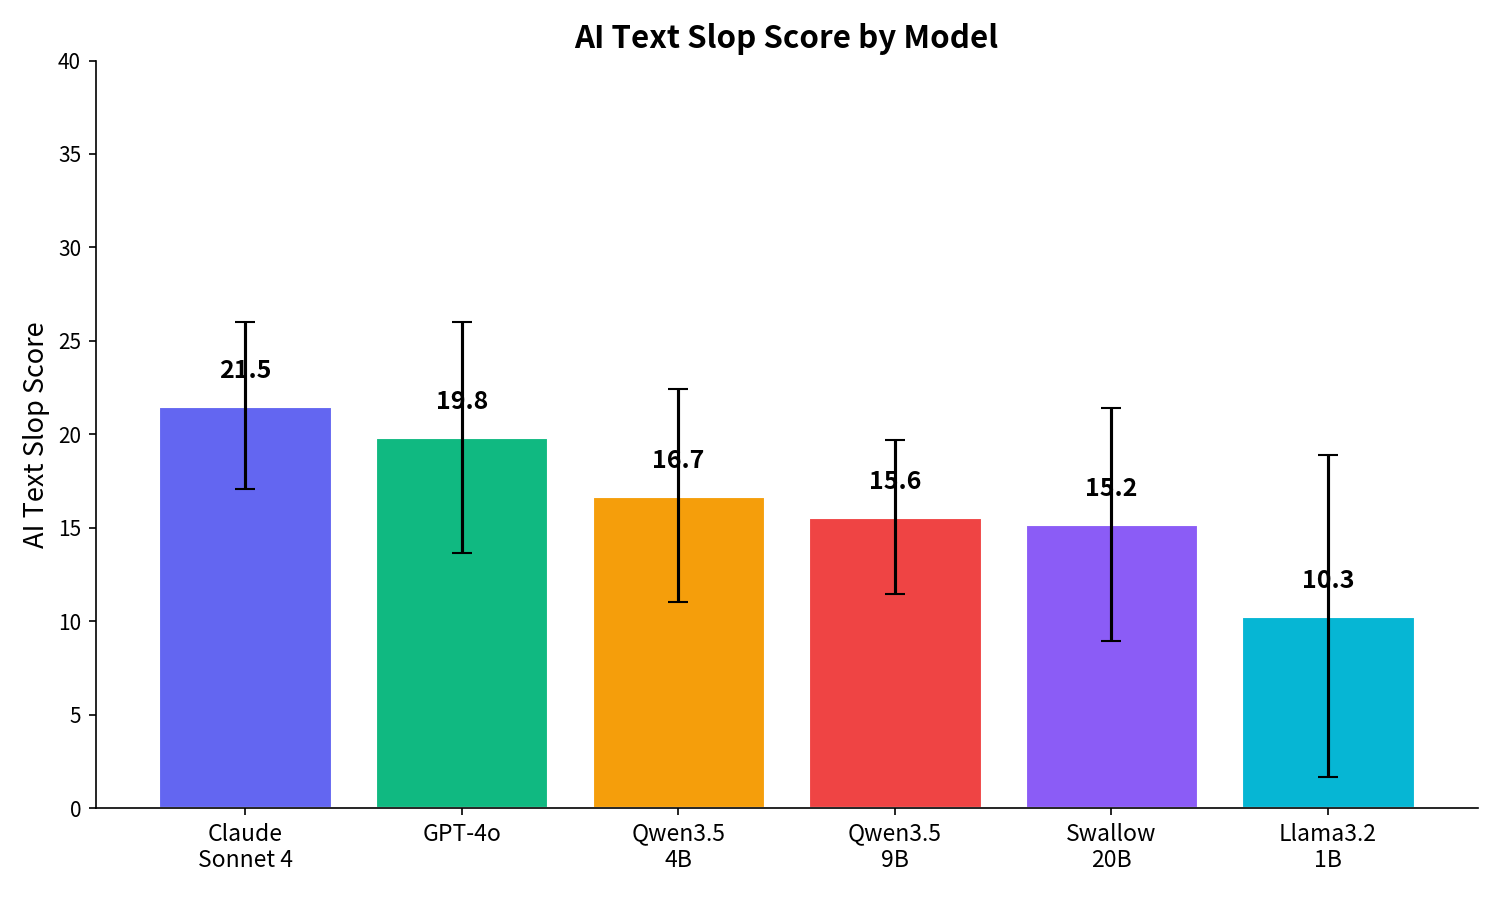
\includegraphics[width=0.85\textwidth]{figures/slop_score_comparison.png}
\caption{AI Text Slop Score by model ($\pm$ 1 SD). Higher scores indicate stronger stylistic convergence toward ``AI-like'' patterns. Commercial models (Claude Sonnet~4, GPT-4o) score significantly higher than open-source alternatives.}
\label{fig:slop_score}
\end{figure}

Figure~\ref{fig:slop_score} shows the composite AI Text Slop Score. Claude Sonnet~4 scores highest ($21.5 \pm 4.5$), followed by GPT-4o ($19.8 \pm 6.3$). The open-source models cluster lower: Qwen~3.5-4B ($16.7 \pm 5.8$), Qwen~3.5-9B ($15.6 \pm 4.2$), Swallow-20B ($15.2 \pm 6.3$), and Llama~3.2-1B ($10.3 \pm 8.8$).

A Kruskal--Wallis test confirms that differences across all six models are statistically significant ($H = 49.87$, $p = 1.47 \times 10^{-9}$). Grouping models into commercial (Claude Sonnet~4 + GPT-4o, mean $= 20.7$) and open-source (Qwen~3.5 + Swallow + Llama, mean $= 14.4$), a Mann--Whitney $U$ test shows that commercial models score significantly higher ($U = 5530$, $p = 2.38 \times 10^{-9}$, Cohen's $d = 1.01$---a large effect). The pairwise comparison between the highest and lowest scoring models (Claude Sonnet~4 vs.\ Llama~3.2-1B) is also highly significant ($U = 786$, $p = 3.52 \times 10^{-7}$).

These results are consistent with the hypothesis that RLHF-based instruction tuning contributes substantially to stylistic convergence, though the observational design does not permit causal claims.

Table~\ref{tab:feature_effects} provides feature-level effect sizes between commercial and open-source models.

\begin{table}[H]
\centering
\caption{Feature-level effect sizes (Cohen's $d$) for commercial vs.\ open-source models. Features marked with *** are significant at $p < 0.001$.}
\label{tab:feature_effects}
\small
\begin{tabular}{lrrrl}
\toprule
\textbf{Feature} & \textbf{Commercial} & \textbf{OSS} & \textbf{$d$} & \textbf{Sig.} \\
\midrule
AI vocabulary & 3.38 & 1.91 & +0.74 & *** \\
Boilerplate concl. & 0.92 & 0.63 & +0.53 & *** \\
Headings & 12.32 & 7.22 & +0.90 & *** \\
List markers & 11.10 & 4.08 & +1.00 & *** \\
Three-set & 1.23 & 0.89 & +0.49 & ** \\
Hedging & 0.35 & 0.20 & +0.24 & ns \\
Bold usage & 7.50 & 8.53 & $-$0.14 & ns \\
Sent.\ length CV & 0.56 & 0.75 & $-$0.41 & ns \\
\bottomrule
\end{tabular}
\end{table}

The strongest discriminators are list markers ($d = +1.00$) and headings ($d = +0.90$), both structural features. At the vocabulary level, AI-frequent vocabulary ($d = +0.74$) is the most discriminating feature. Notably, bold usage and sentence-length CV show no significant difference or favor OSS models, underscoring that the commercial--OSS gap is driven by specific structural and vocabulary features rather than a uniform elevation across all indicators.

\subsection{Pattern Profiles}

\begin{figure}[H]
\centering
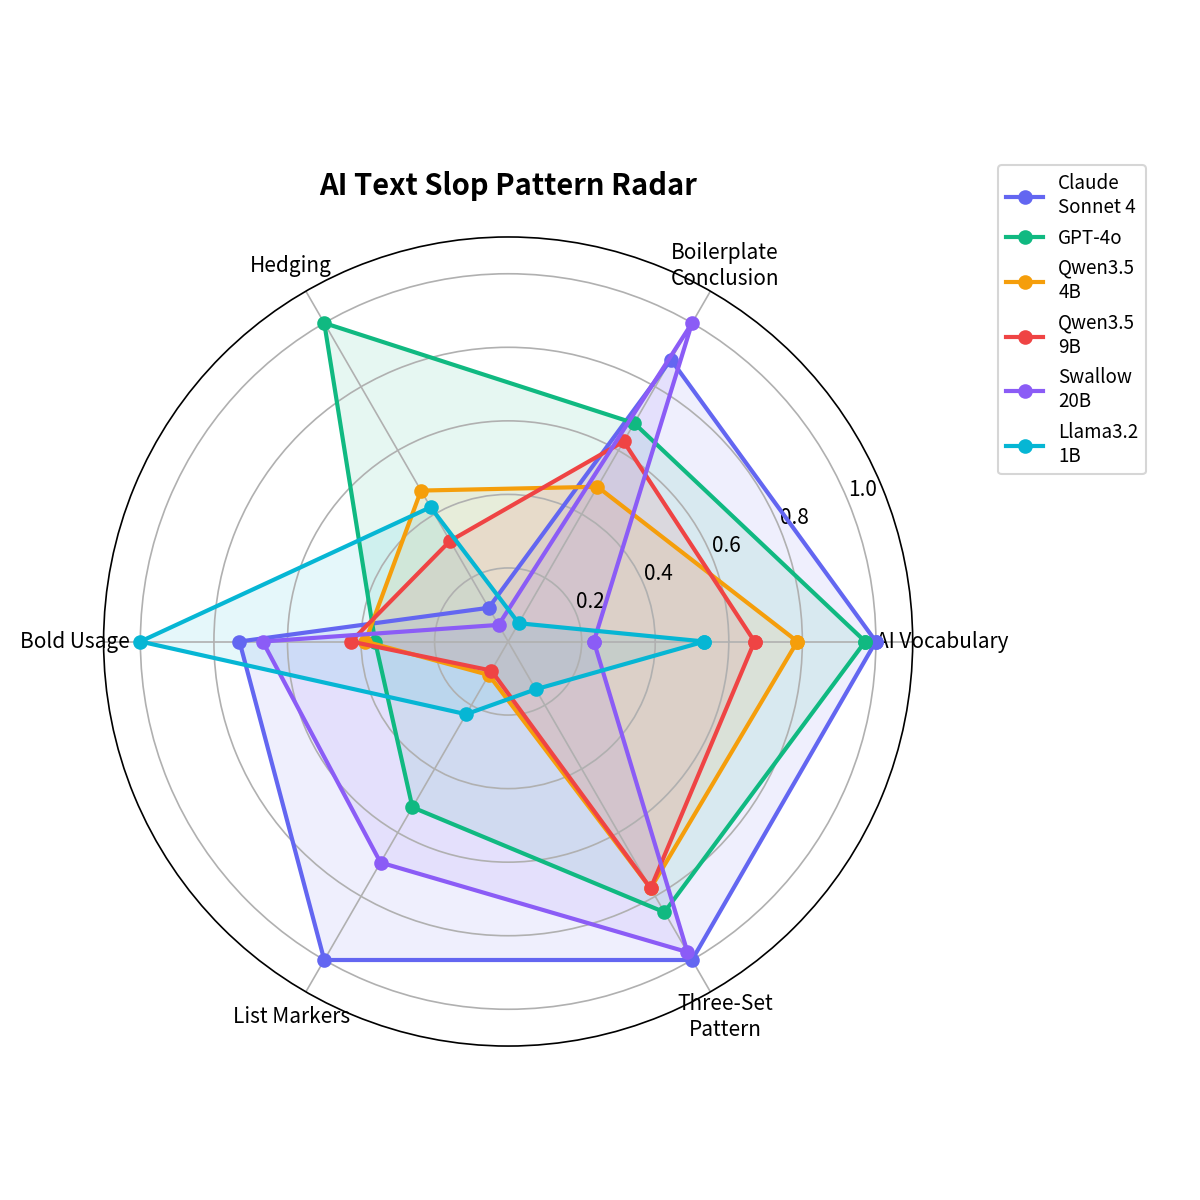
\includegraphics[width=0.85\textwidth]{figures/slop_radar_chart.png}
\caption{Radar chart of normalized pattern indicators. Each model exhibits a distinct ``fingerprint'': Claude Sonnet~4 dominates in AI vocabulary and list markers, while Llama~3.2-1B scores high only on bold usage.}
\label{fig:radar}
\end{figure}

The radar chart (Figure~\ref{fig:radar}) reveals that models do not converge in the same way. Claude Sonnet~4 and GPT-4o are high on AI vocabulary and structural patterns (lists, headings), while Swallow-20B shows a distinctive profile: low AI vocabulary but high boilerplate conclusions and three-set usage.

\subsection{Pattern Heatmap}

\begin{figure}[H]
\centering
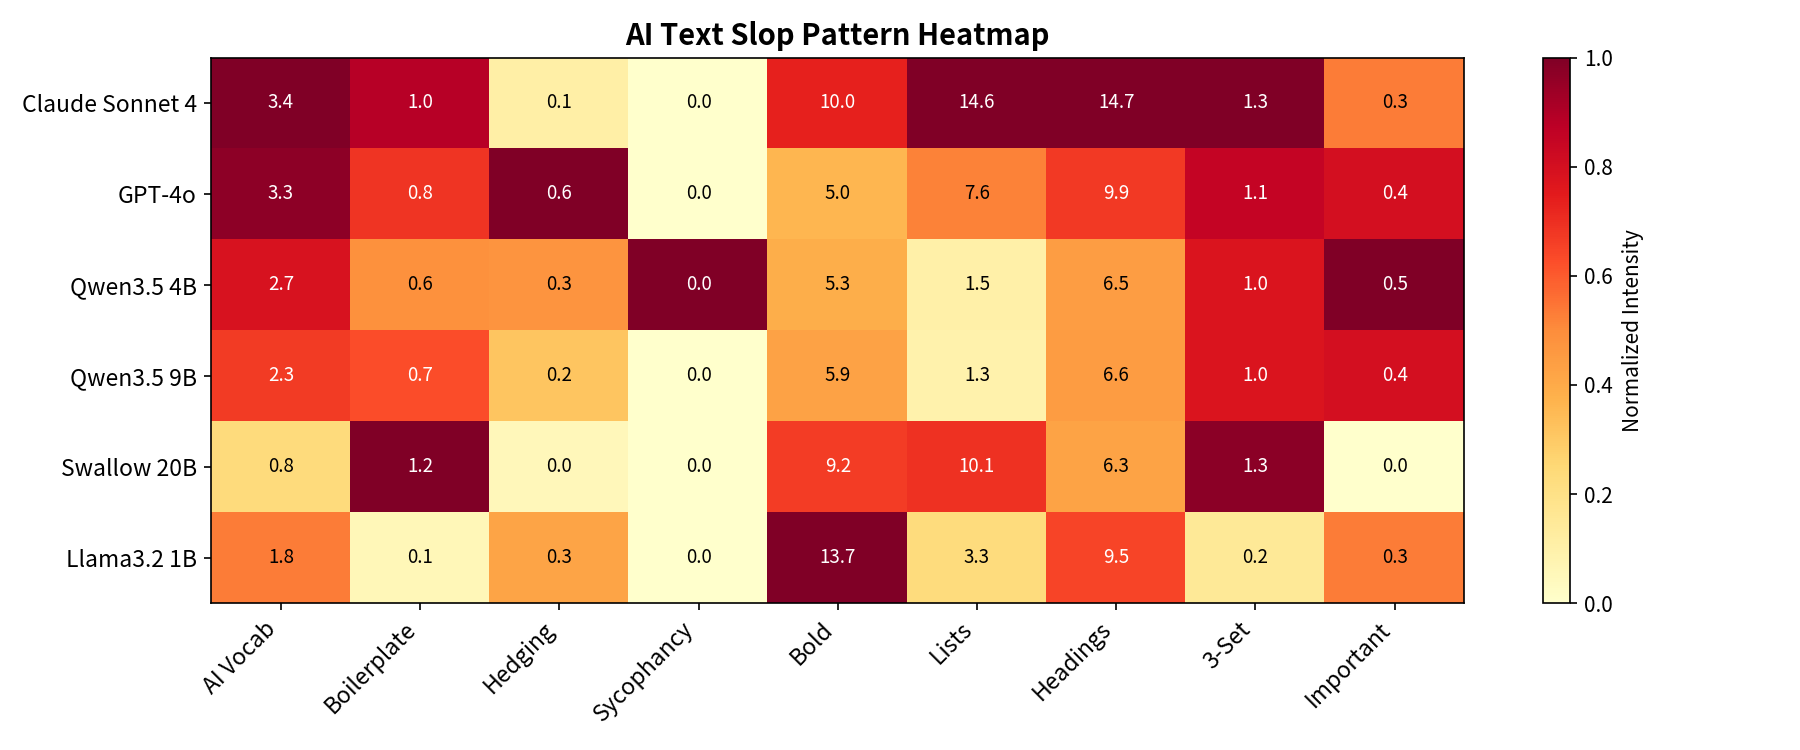
\includegraphics[width=0.95\textwidth]{figures/slop_heatmap.png}
\caption{Heatmap of pattern indicators (normalized by column maximum). Red intensity indicates higher relative usage of each pattern.}
\label{fig:heatmap}
\end{figure}

The heatmap (Figure~\ref{fig:heatmap}) provides a compact view of model-pattern relationships. Key observations:

\begin{itemize}
    \item \textbf{Claude Sonnet~4} is the most ``red'' across multiple columns, reflecting its position as the highest-scoring model.
    \item \textbf{GPT-4o} shows the strongest hedging behavior (0.63 vs.\ $<0.30$ for all other models), a distinctive marker.
    \item \textbf{Swallow-20B} shows bright red in boilerplate conclusions despite near-zero AI vocabulary---a dissociation discussed in Section~5.2.
    \item \textbf{Llama~3.2-1B} is pale across most columns except bold usage, consistent with its lowest Slop Score.
\end{itemize}

\subsection{Text Length Distribution}

\begin{figure}[H]
\centering
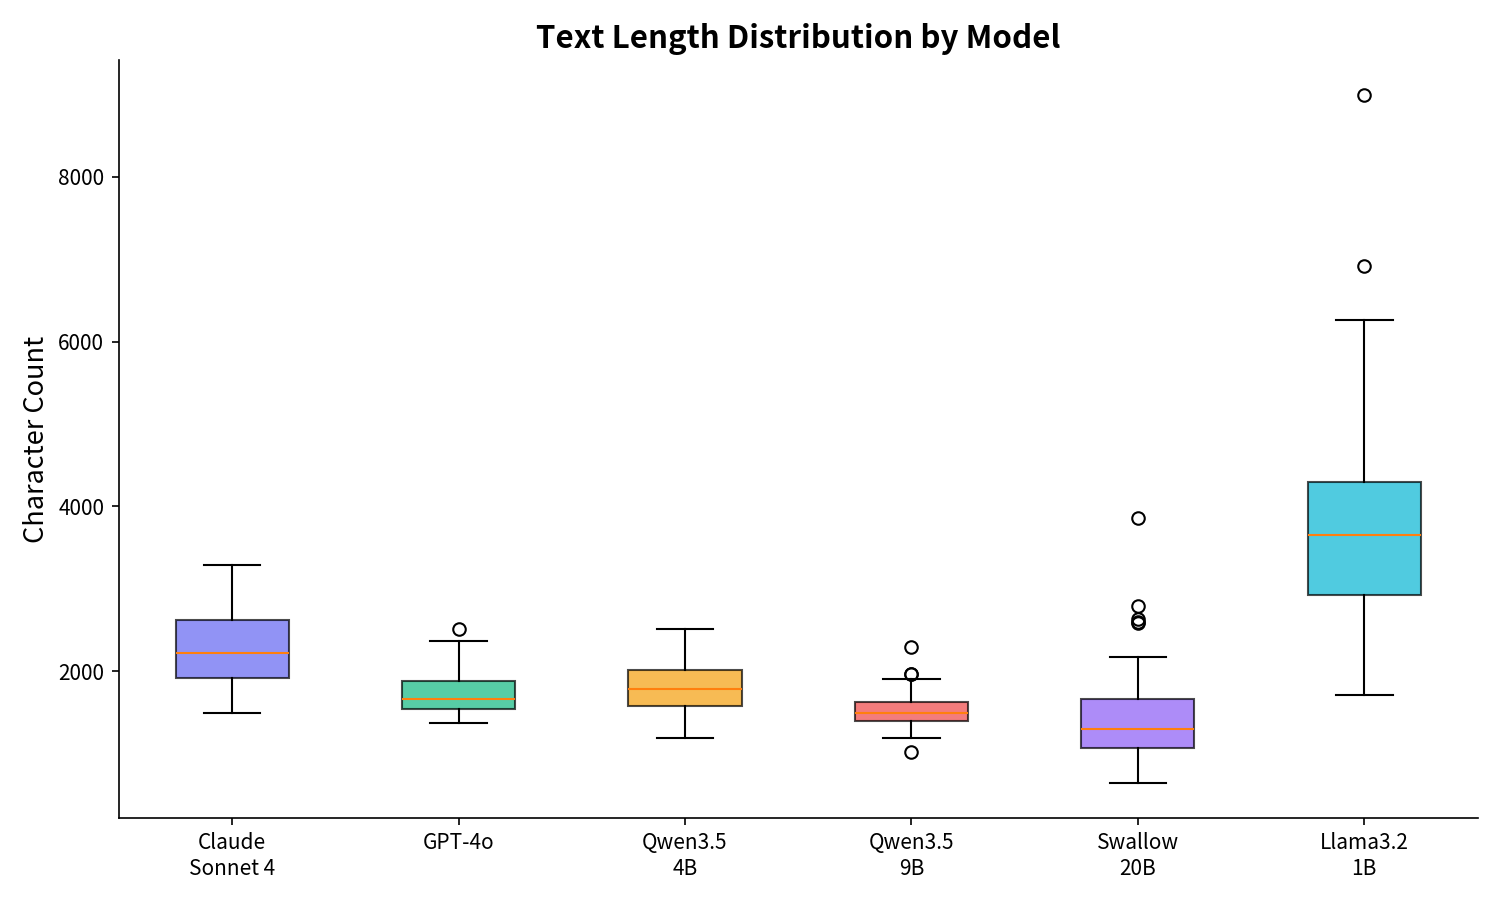
\includegraphics[width=0.75\textwidth]{figures/char_count_boxplot.png}
\caption{Character count distribution by model. All models were prompted for $\sim$800 characters. Llama~3.2-1B dramatically overshoots (median $\sim$3,900), while others cluster around 1,500--2,300.}
\label{fig:boxplot}
\end{figure}

Despite identical prompts requesting approximately 800 characters, output lengths vary dramatically (Figure~\ref{fig:boxplot}). Llama~3.2-1B produces a mean of 3,897 characters (4.9$\times$ the target), suggesting limited instruction-following capability at the 1B parameter scale. Interestingly, no model produces output close to the requested 800 characters; the ``800-ji teido'' (approximately 800 characters) instruction may function as a soft lower bound rather than a strict target for all models tested.

\subsection{Human Baseline Comparison}

To contextualize our AI measurements, we collected 10 human-written Qiita articles on the same topics (one per topic) and applied identical indicators. Table~\ref{tab:human} shows key comparisons.

\begin{table}[H]
\centering
\caption{Human baseline (10 Qiita articles) vs.\ AI models on selected indicators.}
\label{tab:human}
\begin{tabular}{lrrrr}
\toprule
\textbf{Indicator} & \textbf{Human} & \textbf{Claude S4} & \textbf{GPT-4o} & \textbf{Swallow} \\
\midrule
AI vocabulary & 2.70 & \textbf{3.43} & 3.33 & 0.80 \\
Boilerplate concl. & \textbf{2.20} & 1.03 & 0.80 & 1.17 \\
Bold usage & \textbf{13.60} & 10.03 & 4.97 & 9.17 \\
List markers & \textbf{31.80} & 14.60 & 7.60 & 10.13 \\
Headings & \textbf{22.40} & 14.73 & 9.90 & 6.27 \\
Sent.\ length CV & 0.62 & 0.56 & 0.56 & \textbf{0.76} \\
\bottomrule
\end{tabular}
\end{table}

This comparison yields the study's most methodologically important finding: the composite Slop Score for human articles ($28.5 \pm 8.1$) exceeds all AI models, including Claude Sonnet~4 ($21.5 \pm 4.5$). Rather than undermining the score's validity, this result reveals a fundamental distinction between two types of indicators in our framework.

\textbf{Structural indicators} (headings, list markers, boilerplate conclusions) reflect \textit{platform conventions}: Qiita authors routinely use 22.4 headings and 31.8 list markers per article as part of the platform's established ``good article'' template. These patterns predate AI-generated content and are culturally rather than computationally driven.

\textbf{Vocabulary-level indicators}, by contrast, discriminate effectively: Claude Sonnet~4 (3.43) and GPT-4o (3.33) use significantly more AI-characteristic vocabulary than human writers (2.70) and Swallow-20B (0.80).

We therefore characterize our human data as a \textit{preliminary human reference set} rather than a formal control group, given the small sample size ($n = 10$) and single-platform sourcing. Future work should expand to multi-platform comparisons (Qiita, Zenn, note, Hatena Blog) with topic-matched, length-controlled sampling and publication-date stratification. The key implication is that future AI text scoring systems should separate vocabulary-specific sub-scores (which discriminate AI from human) from structural sub-scores (which reflect platform culture) to avoid cultural confounding.

\subsection{Model Scale Effects}

Comparing models by parameter count reveals a non-linear relationship:

\begin{table}[H]
\centering
\caption{Slop Score vs.\ parameter count. RLHF alignment (marked with $\dagger$) appears to matter more than scale.}
\label{tab:scale}
\begin{tabular}{lrrr}
\toprule
\textbf{Model} & \textbf{Parameters} & \textbf{RLHF} & \textbf{Slop Score} \\
\midrule
Llama 3.2-1B & 1B & Minimal & 10.3 \\
Qwen 3.5-4B & 4B & Moderate & 16.7 \\
Qwen 3.5-9B & 9B & Moderate & 15.6 \\
Swallow-20B & 20B & Moderate & 15.2 \\
GPT-4o$^\dagger$ & $\sim$200B (est.) & Extensive & 19.8 \\
Claude Sonnet 4$^\dagger$ & Unknown & Extensive & 21.5 \\
\bottomrule
\end{tabular}
\end{table}

Among the open-source models (1B--20B), the Slop Score does \textit{not} increase monotonically with scale: Qwen~3.5-4B (16.7) scores higher than both Qwen~3.5-9B (15.6) and Swallow-20B (15.2). The largest jump occurs between open-source and commercial models, both of which undergo extensive RLHF. This pattern is consistent with the hypothesis that \textit{alignment training intensity}, rather than model size alone, is a primary factor associated with stylistic convergence.

\section{Discussion}

\subsection{Why Might RLHF Amplify Stylistic Convergence?}

Our results show an association between RLHF alignment intensity and stylistic convergence, consistent with the following mechanism. RLHF training optimizes for human preference ratings \cite{ouyang2022}. Human raters tend to prefer responses that are well-structured, comprehensive, and ``professional''---characteristics that map directly onto our measured patterns: headings for organization, lists for scannability, bold for emphasis, and hedging for epistemic humility. Over many training iterations, this is consistent with distributional convergence \cite{bommasani2021} toward a narrow band of ``approved'' styles.

We emphasize that our observational design establishes correlation rather than causation: commercial models differ from open-source models in many dimensions beyond RLHF (e.g., training data scale, architecture, post-training procedures), and isolating the specific contribution of RLHF would require controlled ablation studies.

This is not merely a cosmetic issue. When all AI-generated text converges on the same style, it becomes:
\begin{itemize}
    \item \textbf{Detectable}: Readers develop intuitions for ``AI voice,'' eroding trust even in high-quality content.
    \item \textbf{Homogenizing}: Platform diversity decreases as AI-assisted authors inadvertently adopt identical styles.
    \item \textbf{Self-reinforcing}: As AI-generated text enters training corpora, future models learn an even narrower style distribution.
\end{itemize}

The feature-level analysis (Table~\ref{tab:feature_effects}) further specifies which indicators drive the gap: structural features (headings $d = 0.90$, lists $d = 1.00$) contribute more than vocabulary ($d = 0.74$), and some indicators (bold usage, sentence-length CV) show no significant commercial--OSS difference at all. This heterogeneity argues against a monolithic ``RLHF effect'' and instead suggests that alignment training may selectively amplify certain structural conventions while leaving other dimensions largely unaffected.

\subsection{The Swallow Paradox}: Low Vocabulary, High Structure}

Swallow-20B presents a striking dissociation: it has the lowest AI-frequent vocabulary count (0.80, vs.\ 3.43 for Claude) yet the highest boilerplate conclusion rate (1.17). We hypothesize this reflects the Japanese-specialized training corpus: Swallow learned more natural Japanese vocabulary from its curated corpus but also internalized the structural conventions (``\textit{ikaga deshita deshou ka},'' ``\textit{matome}'') prevalent in Japanese technical blog culture.

This suggests that vocabulary-level AI detection is insufficient for Japanese text. Structural and rhythmic patterns may be more reliable indicators, particularly for Japanese-specialized models.

\subsection{The Llama Anomaly: Undertrained Models as Style Outliers}

Llama~3.2-1B's dramatically lower Slop Score (10.3) and extreme text length (3,897 characters) are best understood as \textit{insufficient instruction-following} rather than superior writing quality. The model cannot reliably follow length constraints, produces inconsistent formatting, and shows high sentence-length variance ($\text{CV} = 1.08$). Ironically, this ``incompetence'' makes it the least AI-detectable by style metrics---a finding with implications for detection systems that rely on stylistic regularity.

\subsection{Practical Implications}

For writers and editors on Japanese technical platforms:

\begin{enumerate}
    \item \textbf{Vary sentence rhythm}: Deliberately alternate short and long sentences to break the uniform cadence of AI text ($\text{CV} > 0.7$ is more human-like).
    \item \textbf{Avoid boilerplate conclusions}: ``\textit{Ikaga deshita deshou ka}'' (How was it?) is the single strongest AI signal in Japanese text. Replace with original conclusions.
    \item \textbf{Reduce structural scaffolding}: AI overuses headings (14.7/article for Claude vs.\ human norm of 3--5). Use prose transitions instead.
    \item \textbf{Use specific vocabulary}: Replace generic phrases (``\textit{samazama na},'' ``\textit{kouritsuteki na}'') with precise, domain-specific language.
\end{enumerate}

For AI detection tool developers:

\begin{enumerate}
    \item Japanese-language detection should weight \textit{structural} patterns (boilerplate conclusions, three-set, heading density) more heavily than vocabulary-level features, given the Swallow-20B finding.
    \item Multi-dimensional analysis (our 16-indicator approach) outperforms single-feature classifiers, as different models exhibit different pattern profiles.
\end{enumerate}

\subsection{Limitations}

\begin{enumerate}
    \item Our study uses a single prompt template. Varying prompt instructions (e.g., ``write casually'' vs.\ ``write formally'') would likely alter pattern distributions.
    \item Three trials per condition provides limited statistical power. Future work should increase to 10+ trials for robust significance testing.
    \item We analyze only technical blog articles. Other genres (news, creative writing, academic papers) may show different patterns.
    \item The 16 indicators and their weights were defined by the authors. Empirical weight optimization using human-labeled training data would strengthen the Slop Score's validity.
    \item Our human baseline (10 Qiita articles) is limited in size and sampled from a single platform. A larger, multi-platform human corpus with controlled topic matching is needed to refine the distinction between AI-specific and platform-specific patterns.
    \item Commercial model parameter counts and training details are undisclosed, limiting mechanistic interpretation.
\end{enumerate}

\section{Conclusion}

We presented the first systematic quantification of AI text stylistic patterns in Japanese technical writing, analyzing 180 samples across six LLMs with 16 pattern indicators. Our key findings are:

\begin{enumerate}
    \item \textbf{Commercial $>$ open-source in stylistic convergence}: RLHF-aligned models (Claude Sonnet~4: 21.5, GPT-4o: 19.8) score significantly higher on our composite measure than open-source alternatives (Llama~3.2-1B: 10.3), confirmed by Kruskal--Wallis ($H = 49.87$, $p < 10^{-9}$) and Mann--Whitney $U$ tests (Cohen's $d = 1.01$).
    \item \textbf{Alignment intensity is associated with convergence more than model scale}: The Slop Score does not increase monotonically with parameters (4B: 16.7, 9B: 15.6, 20B: 15.2), but jumps sharply for extensively RLHF-trained commercial models.
    \item \textbf{Vocabulary and structural patterns dissociate}: Swallow-20B (Japanese-specialized) shows minimal AI vocabulary but maximal boilerplate usage, indicating that language-specialized training affects these dimensions independently.
    \item \textbf{Each model has a detectable ``fingerprint''}: Claude over-structures, GPT hedges, Swallow concludes formulaically, and Llama cannot follow length instructions.
    \item \textbf{Japanese-specific detection requires structural analysis}: Vocabulary-based detection alone is insufficient due to the Swallow paradox.
    \item \textbf{Structural indicators are culturally confounded}: Human Qiita articles score higher on structural metrics (headings, lists) than AI models, indicating that platform conventions must be separated from AI-specific patterns in future scoring systems.
    \item \textbf{Score robustness}: Sensitivity analysis confirms that the commercial--OSS ranking is preserved under equal weights, vocabulary-only, structure-only, and leave-one-feature-out conditions (Cohen's $d$ = 0.67--1.15), indicating that our findings are not artifacts of the specific weight choices.
\end{enumerate}

This work provides empirical evidence and a starting point for Japanese-language AI text style analysis and writing style improvement tools, and contributes to the broader understanding of how instruction tuning shapes the distributional characteristics of LLM output.

\section*{Reproducibility}

All code, prompts, raw samples, analysis scripts, full indicator definitions, and Japanese phrase lists are available at:\\
\url{https://github.com/kenimo49/ai-text-slop}\\
We release the complete indicator definitions and phrase lists in the repository to ensure that all measurements are fully reproducible by independent researchers.

\begin{thebibliography}{99}

\bibitem{macquarie2025}
Macquarie Dictionary.
AI Slop Named 2025 Word of the Year.
\textit{Macquarie Dictionary Blog}, December 2025.
Merriam-Webster.
AI Slop Named 2025 Word of the Year.
\textit{Merriam-Webster Press Release}, December 2025.

\bibitem{imoto2026aiblue}
Imoto, K.
AI Blue: Systematic Color Recognition Bias in Vision-Language Models and Its Implications for AI-Generated UI Design.
\textit{Zenodo}, DOI: 10.5281/zenodo.19159702, March 2026.

\bibitem{liang2024}
Liang, W., Izzo, Z., Zhang, Y., et al.
Monitoring AI-Modified Content at Scale: A Case Study on the Impact of ChatGPT on AI Conference Peer Reviews.
\textit{arXiv preprint arXiv:2403.07183}, 2024.

\bibitem{guo2024}
Guo, B., Zhang, X., Wang, Z., et al.
How Close is ChatGPT to Human Experts? Comparison Corpus, Evaluation, and Detection.
\textit{arXiv preprint arXiv:2301.07597}, 2024.

\bibitem{mitchell2023}
Mitchell, E., Lee, Y., Khazatsky, A., et al.
DetectGPT: Zero-Shot Machine-Generated Text Detection using Probability Curvature.
\textit{Proceedings of ICML}, 2023.

\bibitem{kirchenbauer2023}
Kirchenbauer, J., Geiping, J., Wen, Y., et al.
A Watermark for Large Language Models.
\textit{Proceedings of ICML}, 2023.

\bibitem{bommasani2021}
Bommasani, R., Hudson, D.A., Adeli, E., et al.
On the Opportunities and Risks of Foundation Models.
\textit{arXiv preprint arXiv:2108.07258}, 2021.

\bibitem{ouyang2022}
Ouyang, L., Wu, J., Jiang, X., et al.
Training Language Models to Follow Instructions with Human Feedback.
\textit{Advances in Neural Information Processing Systems (NeurIPS)}, 2022.

\bibitem{nablas2024}
NABLAS Inc.
AI-Generated Text Detection for Japanese.
\url{https://nablas.com}, 2024.

\end{thebibliography}

\end{document}
